\subsection{Robustness During Overloads}\label{RobustnessDuringOverloads}

\begin{frame}{Mythos:}
	\begin{itemize}
		\item Rate Monotonics ist in Overload-Situationen besser vorhersehbar.
	\end{itemize}
\end{frame}

\subsubsection{Permanent Overload}
\begin{frame}{Permanent Overload: Taskset}
	\begin{center}
		\begin{tabular}{c||c|c}
			Task ($\uptau_i$) & Dauer ($C_i$) & Task-Periode ($T_i$)\\\hline\hline
			$\uptau_1$ & 4 & 8\\
			$\uptau_2$ & 6 & 12\\
			$\uptau_3$ & 5 & 20
		\end{tabular}
		
	\end{center}
\end{frame}

\begin{frame}{Permanent Overload: Rate Monotonics}
\begin{itemize}
			\item $U=(\frac{4}{8}+1)(\frac{6}{12}+1)(\frac{5}{20}+1)\approx 2.81 \nleq 2$\pause		
		\end{itemize}				

		\begin{figure}[htbp]
	% Partly taken from http://www.texample.net/tikz/examples/convolution-of-two-functions/
	\centering
	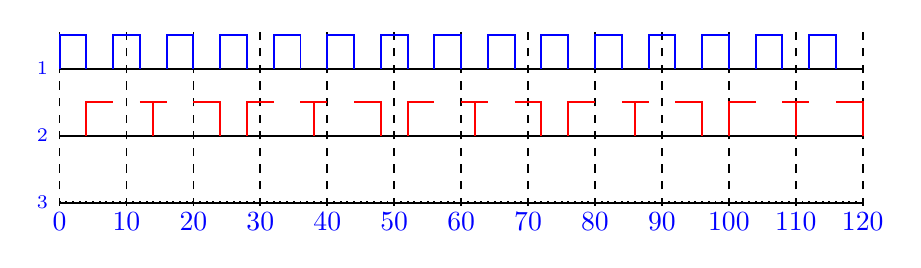
\begin{tikzpicture}[
		scale=0.085,
		line width=0.25mm,
		every node/.style={scale=1, text=blue},
		major tick/.style={semithick, dashed},
		x tick label/.style={anchor=north, minimum width=5mm},
		task1/.style={blue},
		task2/.style={red},
		task3/.style={green},
		desc/.style={anchor=east}
		]


	% Task 3
	\draw (0, 0) -- (120, 0);
	\node[desc] at (0, 0) {$\uptau_3$};
	
	% Task 2
	\draw (0, 10) -- (120, 10);
	\node[desc] at (0, 10) {$\uptau_2$};	

	% Task 1
	\draw (0, 20) -- (120, 20);
	\node[desc] at (0, 20) {$\uptau_1$};	

	
	% Small ticks
	\foreach \x in {0, 1,...,120}{
		\draw (\x, -0.25) -- (\x, 0.25);
	}
	
	% Major ticks with label
	\foreach \x/\label in {0, 10,...,120}{
		\node[x tick label] at (\x, 0) {$\label$}; 		
		\draw[major tick] (\x, -0.5) -- (\x, 26);
	}
	
	% Draw all
	\foreach \x in {0, 24,...,100}{
		\draw[task1] (\x, 20) -- (\x, 25) -- (\x+4, 25) -- (\x+4, 20);
		\draw[task2] (\x+4, 10) -- (\x+4, 15) -- (\x+8, 15);
		\draw[task1] (\x+8, 20) -- (\x+8, 25) -- (\x+12, 25) -- (\x+12, 20);
		\draw[task2] (\x+12, 15) -- (\x+14, 15) -- (\x+14, 10);
		\draw[task2] (\x+14, 10) -- (\x+14, 15) -- (\x+16, 15);
		\draw[task1] (\x+16, 20) -- (\x+16, 25) -- (\x+20, 25) -- (\x+20, 20);
		\draw[task2] (\x+20, 15) -- (\x+24, 15) -- (\x+24, 10);
	}

%	\draw[task1] (0, 10) --  (0, 15) --  (4, 15) -- (4, 10);	

		
	\end{tikzpicture}
%	\caption{Ablaufübersicht}
\end{figure} 
\end{frame}

\begin{frame}{Permanent Overload: Erliest Deadline First}
	\begin{center}
		\begin{itemize}
			\item $U=\frac{4}{8}+\frac{6}{12}+\frac{5}{20}=1.25 \nleq 1$\pause		
		\end{itemize}

	\input{graphics/vergleich/robustness1_EDF.tex}
	\end{center}
\end{frame}

\begin{frame}{Vergleich Permanent Overload}
	\begin{columns}[]
  			\begin{column}{0.5\textwidth}
				Rate Monotonics:
				\begin{itemize}
					\item Tasks mit langer Periode werden vollständig blockiert!
					\item Gut vorhersagbar.
				\end{itemize}

			\end{column}
  			\begin{column}{0.5\textwidth}
  				Erliest Deadline First:
				\begin{itemize}
					\item Sieht chaotischer aus.
					\item Durchschnittliche Periode $\bar{T}_i$ für einen Task $\uptau_i$ ist gegeben durch
						\begin{equation}
							\bar{T}_i=T_i\cdot U
						\end{equation}
				\end{itemize}	
  			\end{column}
	\end{columns}
\end{frame}

%\begin{frame}{\subsubsecname}
%	Beispiel mit EDF? %TODO
%\end{frame}

\begin{frame}{Fazit Permanent Overload:}
	
	\begin{itemize}
		\item Beide Verfahren bei permanenter Überlastung gut vorhersagbar.
		\item Einsatzgebiet ist stark Situationsabhängig.
	\end{itemize}
\end{frame}

\subsubsection{Transient Overload}
\begin{frame}{Annahme für Rate Monotonics:}
	\begin{itemize}
		\item Es werden Tasks mit kurzen Perioden bevorzugt.\pause
		\item[$\Rightarrow$] Falls ein Task seine Deadline überschreitet, wird der Task mit der längsten Periodenlänge verschoben/unterbrochen	.
	\end{itemize}
\end{frame}

\newcommand{\showRMSlideRob}[1] {\begin{frame}{Gegenbeispiel}
	\begin{center}
		\begin{tabular}{c||c|c}
			Task ($\uptau_i$) & Dauer ($C_i$) & Task-Periode ($T_i$)\\\hline\hline
			$\uptau_1$ & 6 & 15\\
			$\uptau_2$ & 9 & 27\\
			$\uptau_3$ & 3 & 60\\
			$\uptau_4$ & 3 & 90
		\end{tabular}
	\end{center}
	\input{graphics/vergleich/transient#1_RM.tex}
	
	\begin{itemize}
		\item[$\Rightarrow$] $\uptau_2$ wird unterbrochen, während Task $\uptau_3$ und $\uptau_4$ nicht beeinflusst werden!
	\end{itemize}
\end{frame}}

\forloop{ct}{7}{\value{ct} < 8}%
{%
	\showRMSlideRob{\arabic{ct}}
}


\begin{frame}{Fazit:}
	\begin{itemize}
		\item Permanent Overload: Gleichwertig.
		\item Transient Overload:
		\begin{itemize}
			\item Rate Monotonics verführt zu falschen Annahmen.
		\end{itemize}
	\end{itemize}
\end{frame}
